\documentclass[11pt]{beamer}
\usetheme{Madrid}
\usepackage[utf8]{inputenc}

 \usepackage[english]{babel}

\usepackage{amsmath}
\usepackage{amsfonts}
\usepackage{amssymb}
\usepackage{graphicx}
\DeclareMathOperator {\argmin}{argmin}

\author{Feichun Yang}
\title{Clustering on Mixed Data}
% Informe o seu email de contato no comando a seguir
% Por exemplo, alcebiades.col@ufes.br
%\setbeamercovered{transparent} 
\setbeamertemplate{navigation symbols}{} 
\logo{
\includegraphics[scale=0.08]{imagens/logomarca_profmat.png}} 
\institute[]{SYRACUSE UNIVERSITY} 
\date{\today} 
%\subject{}

% ---------------------------------------------------------
% Selecione um estilo de referência
\bibliographystyle{apalike}

%\bibliographystyle{abbrv}
%\setbeamertemplate{bibliography item}{\insertbiblabel}
% ---------------------------------------------------------

% ---------------------------------------------------------
% Incluir os slides nos quais as referências foram citadas
%\usepackage[brazilian,hyperpageref]{backref}

%\renewcommand{\backrefpagesname}{Citado na(s) página(s):~}
%\renewcommand{\backref}{}
%\renewcommand*{\backrefalt}[4]{
%	\ifcase #1 %
%		Nenhuma citação no texto.%
%	\or
%		Citado na página #2.%
%	\else
%		Citado #1 vezes nas páginas #2.%
%	\fi}%
% ---------------------------------------------------------

\begin{document}

\begin{frame}
\titlepage
\end{frame}

\begin{frame}{Outline}
\tableofcontents 
\end{frame}

\section{Data}
\begin{frame}{Description}
The data set\cite{palechor2019dataset} consists of information of individuals from countries of Mexico, Peru and Colombia. It contains 17 attributes and 2111 records, labeled with \textbf{NObesity}(Obesity Level). 
The initial collection had 485 records, these data was labeled with:
$$Mass body index = \frac{weight}{height^2}$$
\begin{itemize}
    \item Underweight Less than 18.5
    \item Normal 18.5 to 24.9
    \item Overweight 25.0 to 29.9
    \item Obesity I 30.0 to 34.9
    \item Obesity II 35.0 to 39.9
    \item Obesity III Higher than 40
\end{itemize}
\end{frame} 

\begin{frame}{Description}
    23\% of the data was collected and the remains was generated.

\begin{figure}[!htb]
   \begin{minipage}{0.48\textwidth}
     \centering
     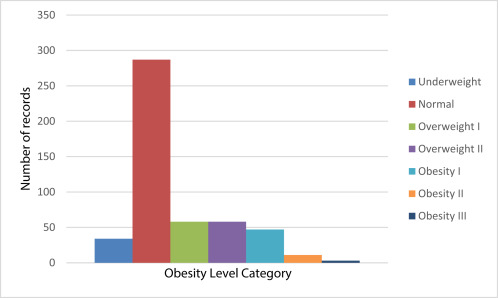
\includegraphics[width=1\linewidth]{images/rawdata.jpg}
     \caption{Before generating}\label{Fig:Data1}
   \end{minipage}\hfill
   \begin{minipage}{0.48\textwidth}
     \centering
     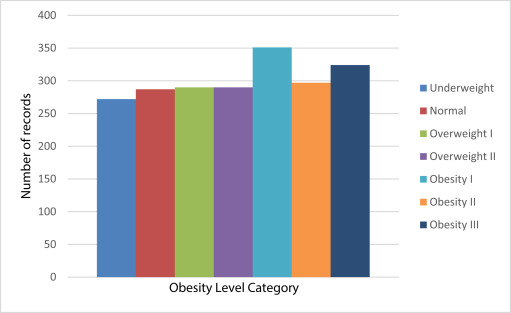
\includegraphics[width=1\linewidth]{images/balanced data.jpg}
     \caption{After generating}\label{Fig:Data2}
   \end{minipage}
\end{figure}


\end{frame}

\begin{frame}{Description}
Continuous Data:
\begin{itemize}
    \item Age
    \item Height(m)
    \item Weight(kg)
    \item FCVC:Frequency of consumption of vegetables(1-3)
    \item NCP: Number of main meals(1-4)
    \item CH2O:Consumption of water daily(1-3)
    \item FAF: Physical activity frequency (0-3)
    \item TUE:Time using technology devices(0-2) 
\end{itemize}

\end{frame}

\begin{frame}{Description}
Categorical Data:
\begin{itemize}
\item Gender(Female/Male)
    \item family\_history\_with\_overweight(No/Yes)
    \item FAVC:Frequent consumption of high caloric food (No/Yes)
    \item CAEC: Consumption of food between meals(no/sometimes/frequently/always) 
    \item SMOKE (No/Yes)
    \item SCC: Calories consumption monitoring(No/Yes)
    \item CALC:Consumption of alcohol(no/sometimes/frequently/always) 
    \item MTRANS:Transportation used (Walking/Bike/Motorbike/Public\_Transportation/Automobile)
    \item NObeyesdad: Obesity level(Insufficient Weight/Normal Weight/Overweight Level I/Overweight Level II/Obesity Type I/Obesity Type II/Obesity Type III)

\end{itemize}
\end{frame}

\begin{frame}{Data Pre-processing}
Goal: Clustering on the dataset of people's eating habits and physical conditions(except height and weight).
\begin{itemize}
    \item Set value to categorical data
    \item Observe the distribution of the numerical variables
\end{itemize}

    \begin{figure}[!htb]
   \begin{minipage}{0.48\textwidth}
     \centering
     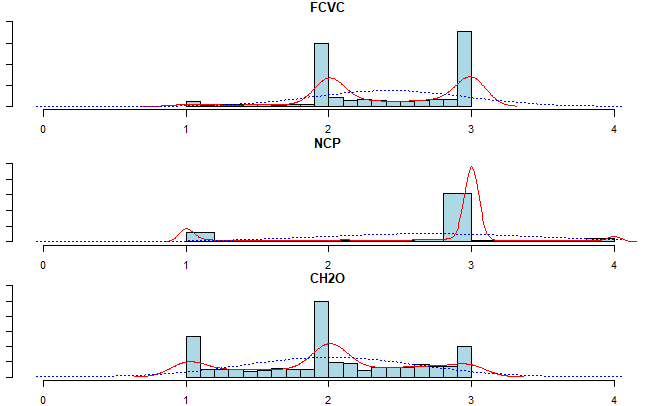
\includegraphics[width=1\linewidth]{images/skew1.png}
     \label{Fig:skew1}
   \end{minipage}\hfill
   \begin{minipage}{0.48\textwidth}
     \centering
     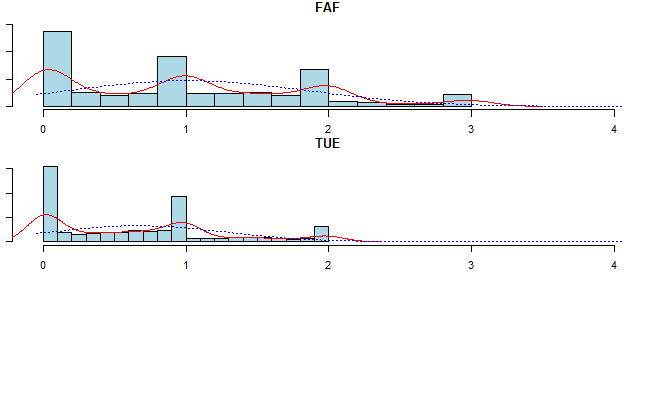
\includegraphics[width=1\linewidth]{images/skew2.png}
     \label{Fig:skew2}
   \end{minipage}
\end{figure}

\end{frame}

\section{Dissimilarity Matrix}
\begin{frame}{Gower Distance}
When the dataset contains different type of data, including logical, numerical, categorical or text data, we can use \textbf{Gower's distance}\cite{gower1971general} to measure the 'distance' between 2 records. 
\begin{figure}
    \centering
    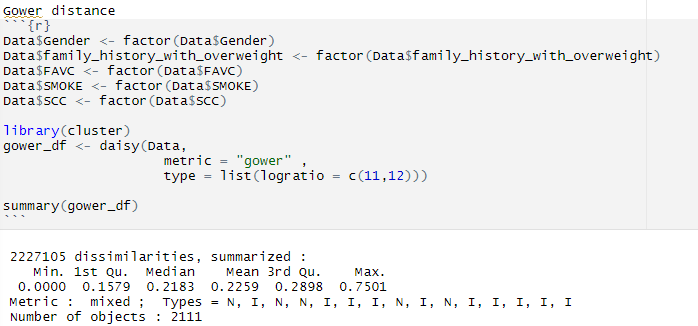
\includegraphics[width=1\linewidth]{images/Gower_dis.png}
    \label{fig:gower}
\end{figure}

\end{frame}

\section{Hierarchical Clustering}
\begin{frame}{Hierarchical Clustering}

    \begin{figure}
        \centering
        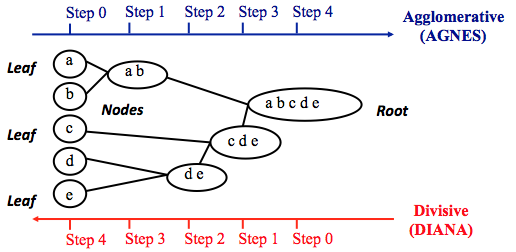
\includegraphics{images/hierarchical-clustering-agnes-diana.png}
        \caption{\cite{boehmke2018uc}}
        \label{fig:hie}
    \end{figure}

    \begin{itemize}
        \item Agglomerative: good at identifyig small clusters
        \item Divisive: good at identifying large clusters
    \end{itemize}
\end{frame}

\begin{frame}{Divisive Clustering}
\begin{figure}
    \centering
    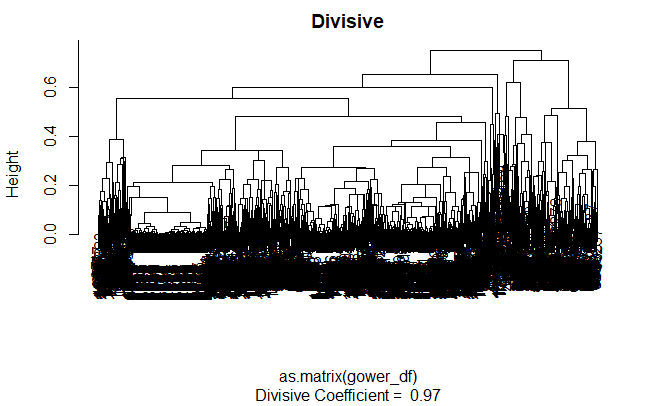
\includegraphics[width=0.8\linewidth]{images/decisive.png}
    \label{fig:my_label}
\end{figure}
Divisive coefficient:$Avg(1-d(i))$, where $d(i)$ is the diameter of the last cluster to which it belongs (before being split off as a single observation), divided by the diameter of the whole dataset.

\end{frame}

\begin{frame}{Agglomerative Clustering}
\begin{figure}
    \centering
    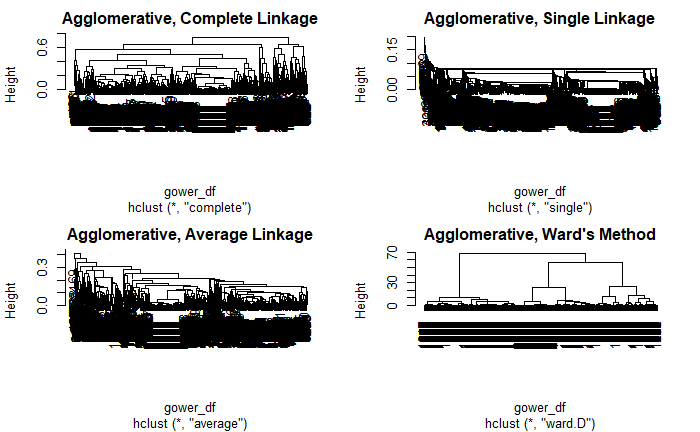
\includegraphics[width=1\linewidth]{images/agglo_comb.png}
    \label{fig:my_label}
\end{figure}
    
\end{frame}

\begin{frame}{Find the Optimal Number of Clusters}
WANT: minimal distance within groups and maximum distance between groups
\begin{itemize}
    \item Elbow Method: minimize the distance within groups
    \item Silhouette Method
\end{itemize}
 \begin{figure}[!htb]
   \begin{minipage}{0.48\textwidth}
     \centering
     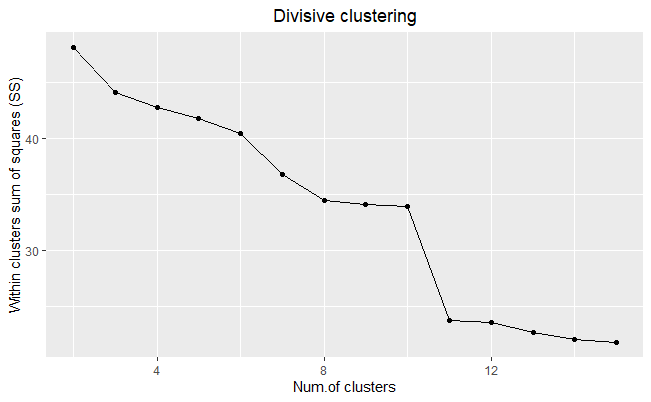
\includegraphics[width=1\linewidth]{images/elbow_for_dec.png}
     \label{Fig:skew1}
   \end{minipage}\hfill
   \begin{minipage}{0.48\textwidth}
     \centering
     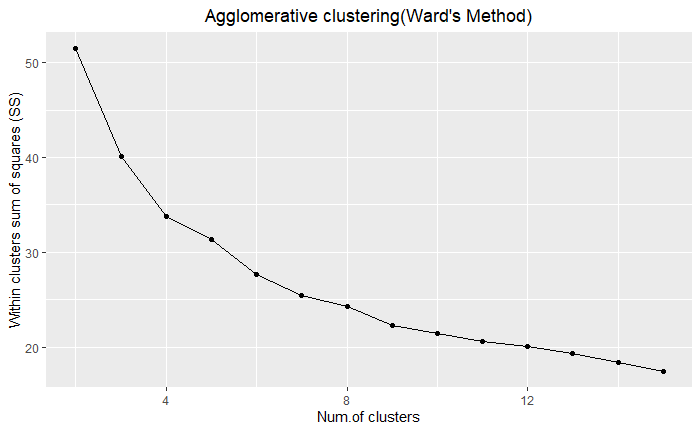
\includegraphics[width=1\linewidth]{elbow_agg_ward.png}
     \label{Fig:skew2}
   \end{minipage}
\end{figure}

\end{frame}

\begin{frame}{Find the Optimal Number of Clusters}
\begin{figure}[!htb]
   \begin{minipage}{0.48\textwidth}
     \centering
     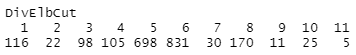
\includegraphics[width=1\linewidth]{images/divcut.png}
     \label{Fig:skew1}
   \end{minipage}\hfill
   \\
   \begin{minipage}{0.48\textwidth}
     \centering
     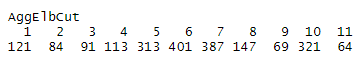
\includegraphics[width=1\linewidth]{images/aggcut.png}
     \label{Fig:skew2}
   \end{minipage}
\end{figure}
Silhouette Method: maximizes the silhouette coefficient, as we want clusters that are distinctive enough to be considered separate.
\begin{figure}[!htb]
   \begin{minipage}{0.48\textwidth}
     \centering
     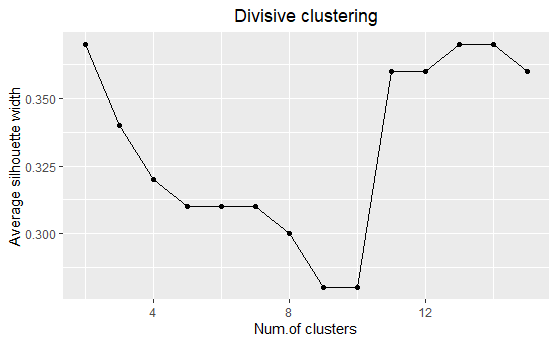
\includegraphics[width=1\linewidth]{images/sil_for_dis.png}
     \label{Fig:skew1}
   \end{minipage}\hfill
   \begin{minipage}{0.48\textwidth}
     \centering
     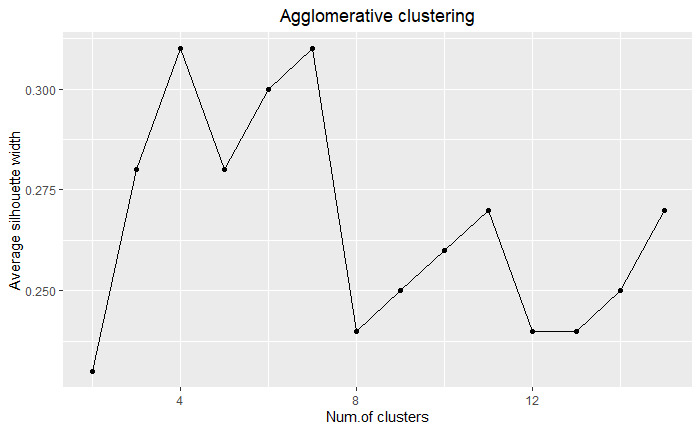
\includegraphics[width=1\linewidth]{images/agg_sil_ward.png}
     \label{Fig:skew2}
   \end{minipage}
\end{figure}

    
\end{frame}

\section{K-medoids Clustering}
\begin{frame}{Partitioning Around Medoids}
PAM is an iterative clustering procedure just like the K-means. Instead of centroids in K-means clustering, PAM iterates over and over until the medoids don't change their positions. The medoid of a cluster is a member of the cluster which is representative of the median of all the attributes under consideration.\cite{bhat2014k}


\end{frame}

\begin{frame}{Silhouette for PAM}
\begin{figure}
    \centering
    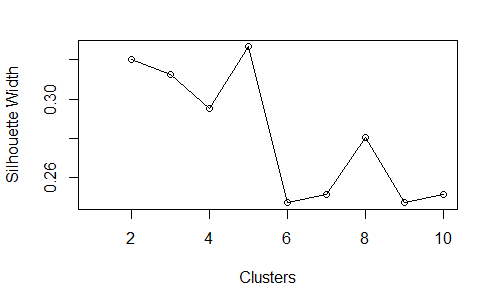
\includegraphics[width=1\linewidth]{images/sil_for_PAM.png}
    \label{fig:my_label}
\end{figure}

\end{frame}

\begin{frame}{Partitioning Around Medoids}
\begin{figure}
\begin{subfigure}{\textwidth}
  \centering
  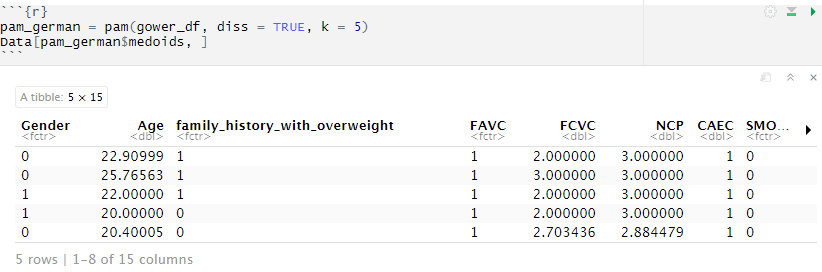
\includegraphics[width=.8\linewidth]{images/Picture4.png}
  
\end{subfigure}%
\begin{subfigure}{\textwidth}
  \centering
  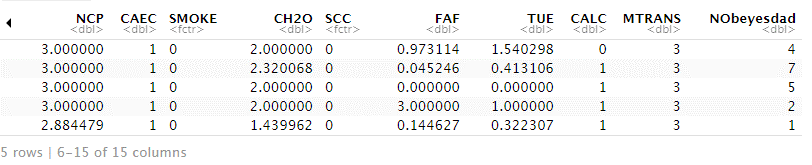
\includegraphics[width=.8\linewidth]{images/Picture5.png}
\end{subfigure}
\end{figure}

\end{frame}

\begin{frame}{Visualize with t-SNE}
\begin{figure}
    \centering
    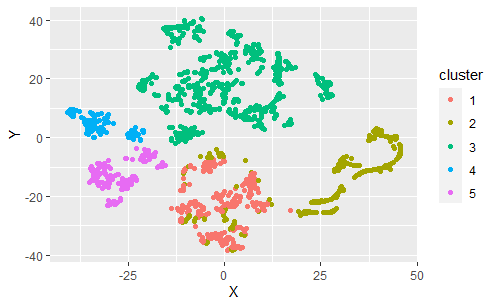
\includegraphics[width=1\linewidth]{images/visualization_pam.png}
    \label{fig:my_label}
\end{figure}

\end{frame}


\section{Reference}
\begin{frame}{Reference}
    \bibliography{referencias}
\end{frame}


\end{document}